\documentclass{standalone}
\usepackage{tikz}
\usetikzlibrary{patterns, positioning}
\usepackage[sfdefault]{ClearSans} %% option 'sfdefault' activates Clear Sans as the default text font
\usepackage[T1]{fontenc}

\begin{document}
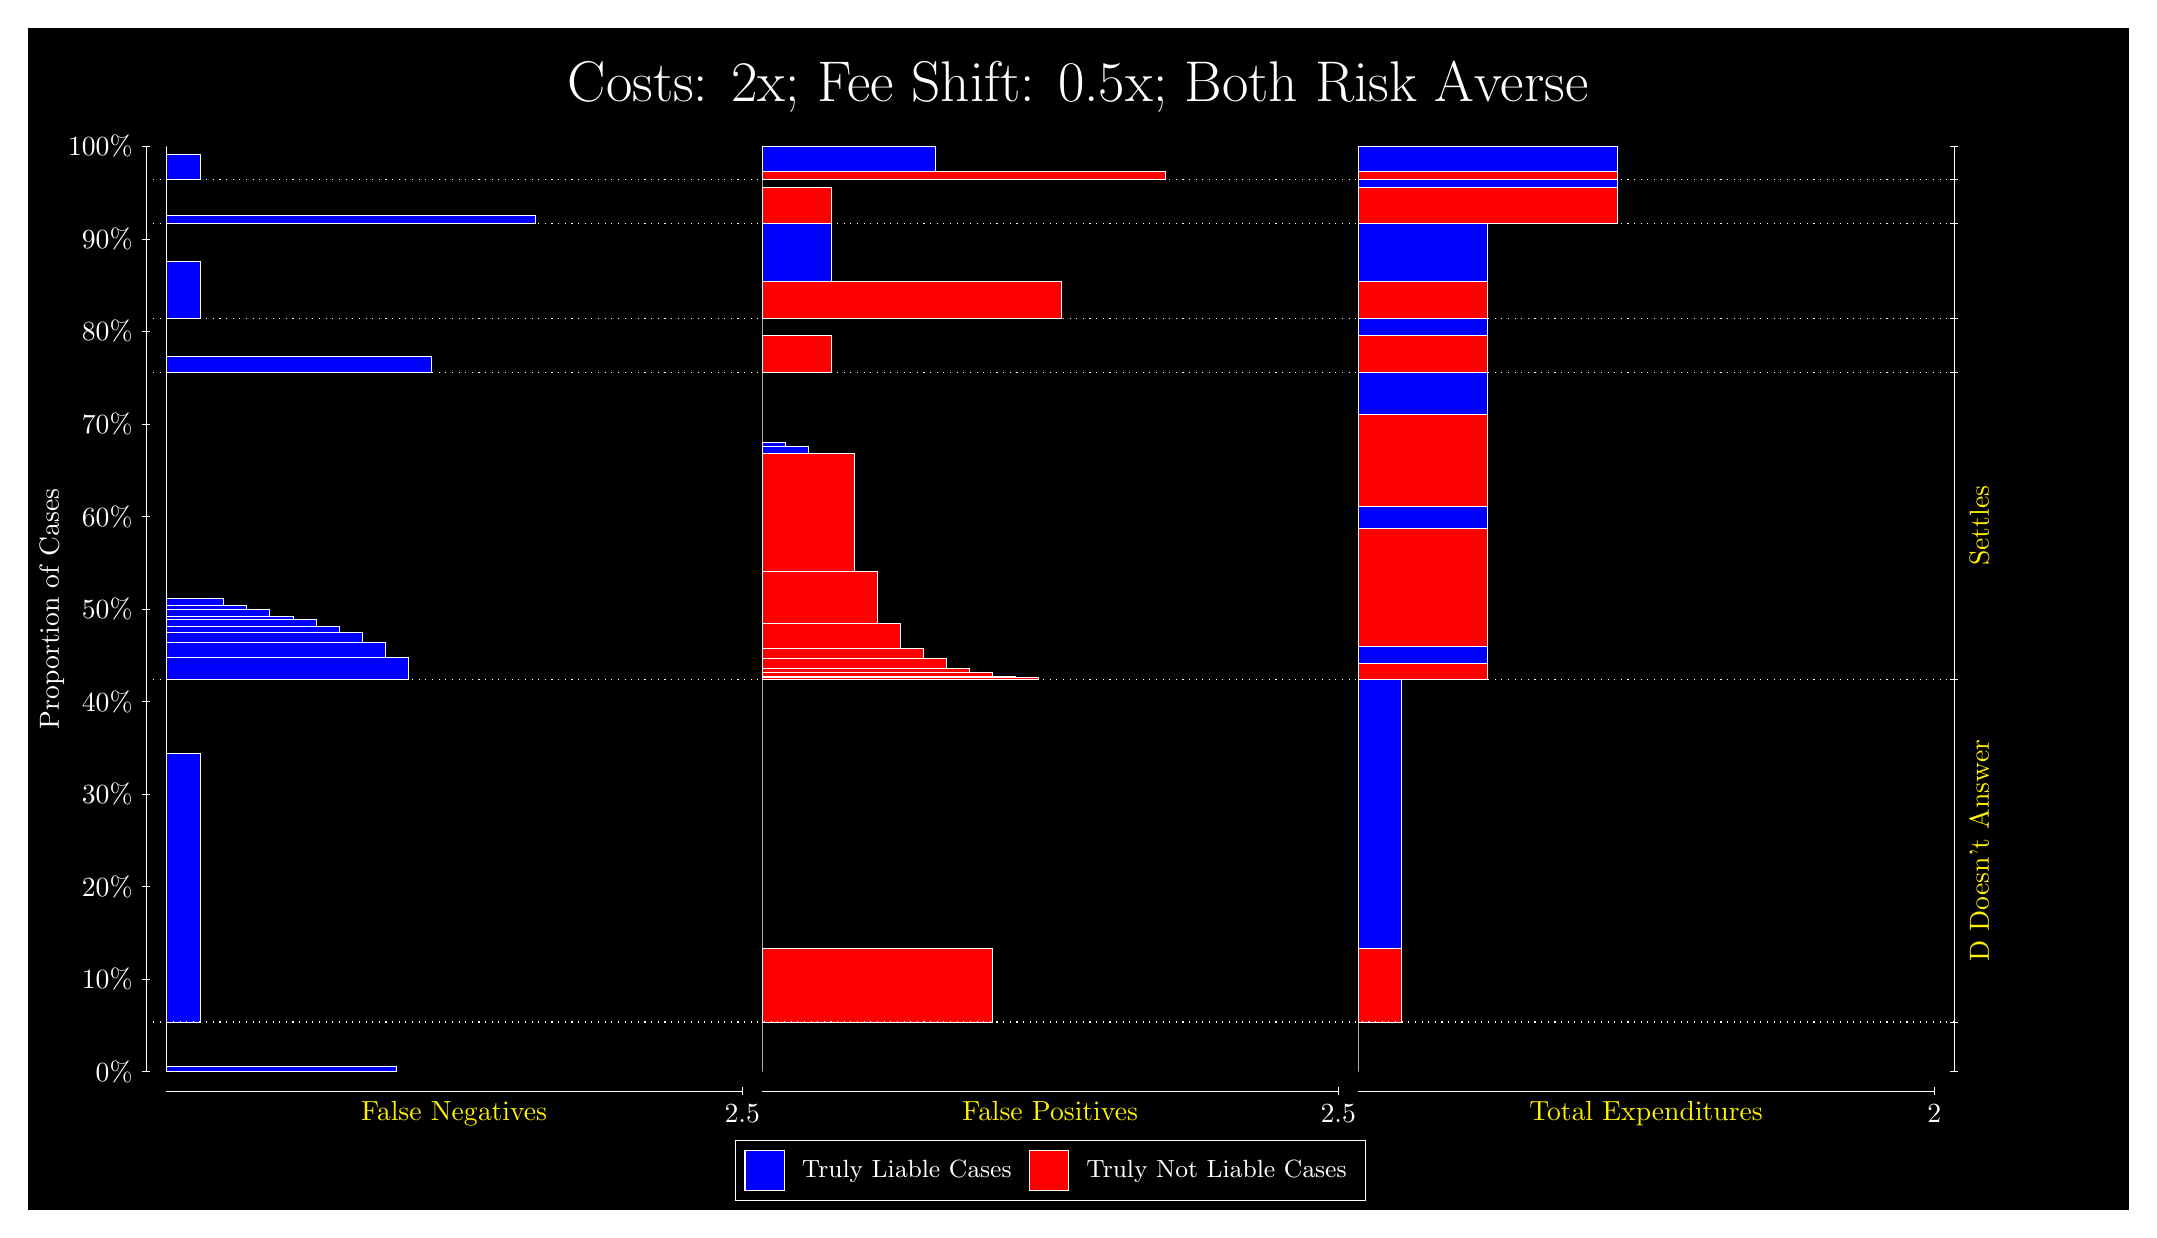
\begin{tikzpicture}
\draw[fill=black] (0,0) rectangle (26.667,15);
\draw[text=white] (0,13.5) rectangle (26.667,15) node[midway] {\huge Costs: 2x; Fee Shift: 0.5x; Both Risk Averse};
\draw[white, very thin] (1.5,1.75) -- (1.5,13.5);
\node[rotate=90, text=white, anchor=center] at (0.3, 7.625) {Proportion of Cases};
\draw[white, very thin] (1.45,1.75) -- (1.55,1.75);
\node[text=white, anchor=east] at (1.45, 1.75) {0\%};
\draw[white, very thin] (1.45,2.925) -- (1.55,2.925);
\node[text=white, anchor=east] at (1.45, 2.925) {10\%};
\draw[white, very thin] (1.45,4.1) -- (1.55,4.1);
\node[text=white, anchor=east] at (1.45, 4.1) {20\%};
\draw[white, very thin] (1.45,5.275) -- (1.55,5.275);
\node[text=white, anchor=east] at (1.45, 5.275) {30\%};
\draw[white, very thin] (1.45,6.45) -- (1.55,6.45);
\node[text=white, anchor=east] at (1.45, 6.45) {40\%};
\draw[white, very thin] (1.45,7.625) -- (1.55,7.625);
\node[text=white, anchor=east] at (1.45, 7.625) {50\%};
\draw[white, very thin] (1.45,8.8) -- (1.55,8.8);
\node[text=white, anchor=east] at (1.45, 8.8) {60\%};
\draw[white, very thin] (1.45,9.975) -- (1.55,9.975);
\node[text=white, anchor=east] at (1.45, 9.975) {70\%};
\draw[white, very thin] (1.45,11.15) -- (1.55,11.15);
\node[text=white, anchor=east] at (1.45, 11.15) {80\%};
\draw[white, very thin] (1.45,12.325) -- (1.55,12.325);
\node[text=white, anchor=east] at (1.45, 12.325) {90\%};
\draw[white, very thin] (1.45,13.5) -- (1.55,13.5);
\node[text=white, anchor=east] at (1.45, 13.5) {100\%};

\draw[white, very thin] (24.457,1.75) -- (24.457,13.5);
\draw[white, very thin] (24.407,1.75) -- (24.507,1.75);
\node[anchor=west] at (24.407, 1.75) {};
\draw[white, very thin] (24.407,2.3784) -- (24.507,2.3784);
\node[anchor=west] at (24.407, 2.3784) {};
\draw[white, very thin] (24.407,6.7317) -- (24.507,6.7317);
\node[anchor=west] at (24.407, 6.7317) {};
\draw[white, very thin] (24.407,10.63) -- (24.507,10.63);
\node[anchor=west] at (24.407, 10.63) {};
\draw[white, very thin] (24.407,11.314) -- (24.507,11.314);
\node[anchor=west] at (24.407, 11.314) {};
\draw[white, very thin] (24.407,12.518) -- (24.507,12.518);
\node[anchor=west] at (24.407, 12.518) {};
\draw[white, very thin] (24.407,13.078) -- (24.507,13.078);
\node[anchor=west] at (24.407, 13.078) {};
\draw[white, very thin] (24.407,13.5) -- (24.507,13.5);
\node[anchor=west] at (24.407, 13.5) {};

\draw[white, very thin, fill=blue] (1.75,1.75) rectangle (4.6775,1.8161);
\draw[white, very thin, fill=red] (1.75,1.8161) rectangle (1.75,2.3784);
\draw[white, very thin, fill=blue] (1.75,2.3784) rectangle (2.1891,5.7927);
\draw[white, very thin, fill=red] (1.75,5.7927) rectangle (1.75,6.7317);
\draw[white, very thin, fill=blue] (1.75,6.7317) rectangle (4.8239,7.0137);
\draw[white, very thin, fill=blue] (1.75,7.0137) rectangle (4.5312,7.2017);
\draw[white, very thin, fill=blue] (1.75,7.2017) rectangle (4.2384,7.3309);
\draw[white, very thin, fill=blue] (1.75,7.3309) rectangle (3.9457,7.4046);
\draw[white, very thin, fill=blue] (1.75,7.4046) rectangle (3.6529,7.4906);
\draw[white, very thin, fill=blue] (1.75,7.4906) rectangle (3.3602,7.5357);
\draw[white, very thin, fill=blue] (1.75,7.5357) rectangle (3.0674,7.6241);
\draw[white, very thin, fill=blue] (1.75,7.6241) rectangle (2.7746,7.673);
\draw[white, very thin, fill=blue] (1.75,7.673) rectangle (2.4819,7.7658);
\draw[white, very thin, fill=red] (1.75,7.7658) rectangle (1.75,10.63);
\draw[white, very thin, fill=blue] (1.75,10.63) rectangle (5.1167,10.838);
\draw[white, very thin, fill=red] (1.75,10.838) rectangle (1.75,11.314);
\draw[white, very thin, fill=blue] (1.75,11.314) rectangle (2.1891,12.044);
\draw[white, very thin, fill=red] (1.75,12.044) rectangle (1.75,12.518);
\draw[white, very thin, fill=blue] (1.75,12.518) rectangle (6.4341,12.621);
\draw[white, very thin, fill=red] (1.75,12.621) rectangle (1.75,13.078);
\draw[white, very thin, fill=blue] (1.75,13.078) rectangle (2.1891,13.398);
\draw[white, very thin, fill=red] (1.75,13.398) rectangle (1.75,13.5);
\draw[white, very thin, fill=red] (9.3189,1.75) rectangle (9.3189,2.3123);
\draw[white, very thin, fill=blue] (9.3189,2.3123) rectangle (9.3189,2.3784);
\draw[white, very thin, fill=red] (9.3189,2.3784) rectangle (12.246,3.3174);
\draw[white, very thin, fill=blue] (9.3189,3.3174) rectangle (9.3189,6.7317);
\draw[white, very thin, fill=red] (9.3189,6.7317) rectangle (12.832,6.7533);
\draw[white, very thin, fill=red] (9.3189,6.7533) rectangle (12.539,6.7752);
\draw[white, very thin, fill=red] (9.3189,6.7752) rectangle (12.246,6.8169);
\draw[white, very thin, fill=red] (9.3189,6.8169) rectangle (11.954,6.865);
\draw[white, very thin, fill=red] (9.3189,6.865) rectangle (11.661,7.0026);
\draw[white, very thin, fill=red] (9.3189,7.0026) rectangle (11.368,7.1312);
\draw[white, very thin, fill=red] (9.3189,7.1312) rectangle (11.075,7.4401);
\draw[white, very thin, fill=red] (9.3189,7.4401) rectangle (10.783,8.1065);
\draw[white, very thin, fill=red] (9.3189,8.1065) rectangle (10.49,9.5961);
\draw[white, very thin, fill=blue] (9.3189,9.5961) rectangle (9.9044,9.6889);
\draw[white, very thin, fill=blue] (9.3189,9.6889) rectangle (9.6116,9.7378);
\draw[white, very thin, fill=blue] (9.3189,9.7378) rectangle (9.3189,10.63);
\draw[white, very thin, fill=red] (9.3189,10.63) rectangle (10.197,11.106);
\draw[white, very thin, fill=blue] (9.3189,11.106) rectangle (9.3189,11.314);
\draw[white, very thin, fill=red] (9.3189,11.314) rectangle (13.125,11.788);
\draw[white, very thin, fill=blue] (9.3189,11.788) rectangle (10.197,12.518);
\draw[white, very thin, fill=red] (9.3189,12.518) rectangle (10.197,12.975);
\draw[white, very thin, fill=blue] (9.3189,12.975) rectangle (9.3189,13.078);
\draw[white, very thin, fill=red] (9.3189,13.078) rectangle (14.442,13.18);
\draw[white, very thin, fill=blue] (9.3189,13.18) rectangle (11.515,13.5);
\draw[white, very thin, fill=red] (16.888,1.75) rectangle (16.888,2.3123);
\draw[white, very thin, fill=blue] (16.888,2.3123) rectangle (16.888,2.3784);
\draw[white, very thin, fill=red] (16.888,2.3784) rectangle (17.437,3.3174);
\draw[white, very thin, fill=blue] (16.888,3.3174) rectangle (17.437,6.7317);
\draw[white, very thin, fill=red] (16.888,6.7317) rectangle (18.534,6.9329);
\draw[white, very thin, fill=blue] (16.888,6.9329) rectangle (18.534,7.1562);
\draw[white, very thin, fill=red] (16.888,7.1562) rectangle (18.534,8.6458);
\draw[white, very thin, fill=blue] (16.888,8.6458) rectangle (18.534,8.9277);
\draw[white, very thin, fill=red] (16.888,8.9277) rectangle (18.534,10.101);
\draw[white, very thin, fill=blue] (16.888,10.101) rectangle (18.534,10.63);
\draw[white, very thin, fill=red] (16.888,10.63) rectangle (18.534,11.106);
\draw[white, very thin, fill=blue] (16.888,11.106) rectangle (18.534,11.314);
\draw[white, very thin, fill=red] (16.888,11.314) rectangle (18.534,11.788);
\draw[white, very thin, fill=blue] (16.888,11.788) rectangle (18.534,12.518);
\draw[white, very thin, fill=red] (16.888,12.518) rectangle (20.181,12.975);
\draw[white, very thin, fill=blue] (16.888,12.975) rectangle (20.181,13.078);
\draw[white, very thin, fill=red] (16.888,13.078) rectangle (20.181,13.18);
\draw[white, very thin, fill=blue] (16.888,13.18) rectangle (20.181,13.5);
\draw[white, dotted] (1.5,2.3784) -- (24.457,2.3784);
\draw[white, dotted] (1.5,6.7317) -- (24.457,6.7317);
\draw[white, dotted] (1.5,10.63) -- (24.457,10.63);
\draw[white, dotted] (1.5,11.314) -- (24.457,11.314);
\draw[white, dotted] (1.5,12.518) -- (24.457,12.518);
\draw[white, dotted] (1.5,13.078) -- (24.457,13.078);
\draw[white, very thin] (1.75,1.5) -- (9.0689,1.5);
\node[text=yellow, anchor=north] at (5.4094, 1.5) {False Negatives};
\draw[white, very thin] (9.0689,1.45) -- (9.0689,1.55);
\node[text=white, anchor=north] at (9.0689, 1.45) {2.5};

\draw[white, very thin] (9.3189,1.5) -- (16.638,1.5);
\node[text=yellow, anchor=north] at (12.978, 1.5) {False Positives};
\draw[white, very thin] (16.638,1.45) -- (16.638,1.55);
\node[text=white, anchor=north] at (16.638, 1.45) {2.5};

\draw[white, very thin] (16.888,1.5) -- (24.207,1.5);
\node[text=yellow, anchor=north] at (20.547, 1.5) {Total Expenditures};
\draw[white, very thin] (24.207,1.45) -- (24.207,1.55);
\node[text=white, anchor=north] at (24.207, 1.45) {2};


\node[text=yellow, centered, rotate=90] at (24.777, 4.5551) {D Doesn't Answer};
\node[text=yellow, centered, rotate=90] at (24.777, 8.681) {Settles};





\draw (12.978300999999998,1.5) node[draw=none] (baseCoordinate) {};
\begin{scope}[align=center]
        \matrix[scale=0.5, draw=white, below=0.5cm of baseCoordinate, nodes={draw}, column sep=0.1cm]{
            \node[rectangle, draw, minimum width=0.5cm, minimum height=0.5cm, fill=blue] {}; &
            \node[draw=none, font=\small, text=white] (B) {Truly Liable Cases}; &
            \node[rectangle, draw, minimum width=0.5cm, minimum height=0.5cm, fill=red] {}; &
            \node[draw=none, font=\small, text=white] (B) {Truly Not Liable Cases}; \\
            };
\end{scope}

\end{tikzpicture}
\end{document}